\section{Exercise 1}

Assuming the following:
\begin{itemize}
    \item All functional units are pipelined.
    \item ALU operations take 1 cycle.
    \item Memory operations take 3 cycles (includes time in ALU).
    \item Floating-point add instructions take 3 cycles.
    \item Floating-point multiply instructions take 5 cycles.
    \item There is no register renaming or forwarding.
    \item Instructions are fetched, decoded, and issued in order.
    \item The ISSUE stage is a buffer of unlimited length that holds instructions waiting to start execution.
    \item An instruction will only enter the issue stage if it does not cause a WAR or WAW hazard.
    \item Only one instruction can be issued at a time, and in the case of multiple instructions being ready, the oldest one will go first.
    \item Program Counter calculation for branches and jumps has been anticipated in the ISSUE stage.
    \item The target address for a branch is available in the FETCH stage.
\end{itemize}
Consider the code:
\begin{verbatim}
I1: FOR: ld $f2, VB($r6)
I2: fadd $f3, $f2, $f6
I3: st $f3, VA($r7)
I4: ld $f3, VC($r6)
I5: st $f3, VC($r7)
I6: fadd $f4, $f4, $f3
I7: addi $r6, $r6, 4
I8: addi $r7, $r7, 4
I9: blt $r7, $r8, FOR
\end{verbatim}
Examine each conflict considering the operation durations:
\begin{itemize}
\item Arithmetic logic unit operations: 1 cycle.
\item Memory operations: 3 cycles.
\item Floating-point addition: 3 cycles.
\item Floating-point multiplication: 5 cycles.
\end{itemize}

\subsection*{Solution}
The conflicts are:
\begin{itemize}
\item RAW:\@ F2 (I1-I2), F3 (I2-I3), F3 (I4-I5), F3 (I4-I6), R7 (I8-I9).
\item WAR:\@ R7 (I8-I5, I8-I3), R6 (I7-I1, I7-I4).
\item WAW:\@ F3 (I2-I4).
\item CNTRL.\@
\end{itemize}
The corresponding pipeline schema is: 
\begin{figure}[H]
    \centering
    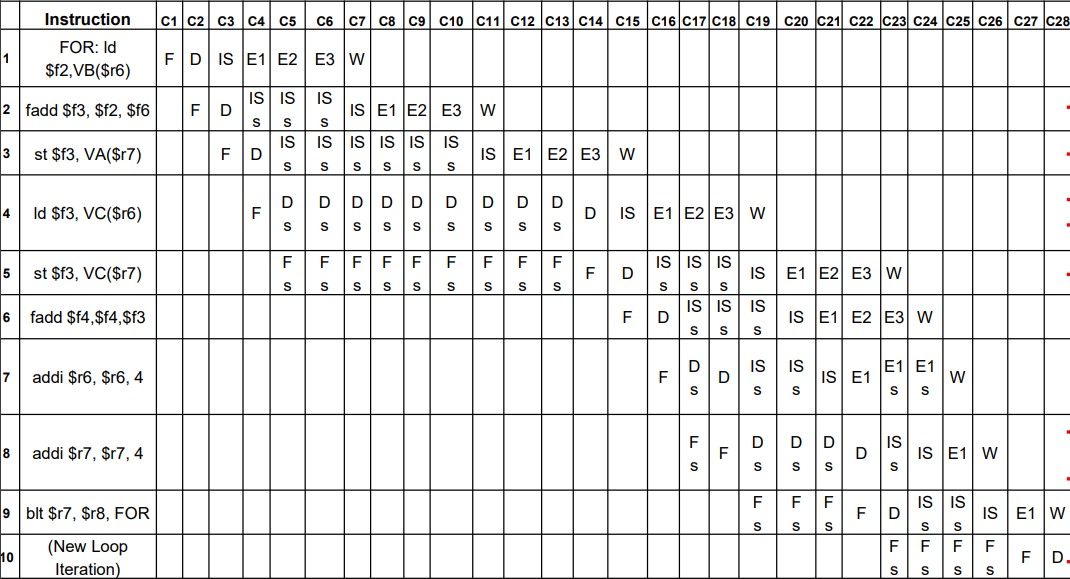
\includegraphics[width=1\linewidth]{images/pip.png}
\end{figure}